\chapter{Distribution of connections\label{ch:nonspatial}}

\graphicspath{{figs/nonspatial/}}



We will now describe a procedure for testing random convergent and divergent connection algorithms for networks without spatial structure. These connection algorithms were described in the introduction, and an example of a resulting network was shown in Figure \ref{fig:rdc_example_intro}.



\section{Random convergent connections\label{sec:rcc}}

For each target node \inline{RandomConvergentConnect} iterates over, it randomly draws $C\label{eq:C}$ source nodes from the $r = N_\text{s}\label{eq:Ns}$ available source nodes and connects to them. Multapses and autapses are allowed, i.e., nodes are drawn with replacement. We are interested in checking whether all the source nodes are drawn with equal probability. In other words, we want to test the observed distribution of connections against the expected uniform distribution. Each drawing of a source node can be thought of as a trial as described in Section \ref{sec:chi}, with exactly \emph{one} outcome $A_i$. The total number of trials is $n = N_\text{t} \times C$, where $N_\text{t}\label{eq:Nt}$ is the number of target neurons. After all $n$ trials, each source node $i$ will have some out-degree (number of outgoing connections), described by the \emph{frequency of outcome $A_i$} as defined in Equation \ref{eq:nui}:
\begin{equation}
\nu_i = \sum_{k=1}^n{\mu_{ki}}.
\end{equation}
The vector of frequencies, 
\begin{equation}
\bm{\nu} = \sum_{k=1}^n{\bm{\mu_k}} = (\nu_1, \nu_2, ..., \nu_r),
\end{equation}
now contains all observed out-degrees. 

In this particular case, the \emph{expected} frequencies are all the same, $\text{E}(\nu_i) = np^{(0)}$, so the vector of expected frequencies contains $r$ equal entries, $\text{E}(\bm{\nu}) = n\bm{p}^{(0)} = (np^{(0)}, np^{(0)}, ..., np^{(0)})$.

To test the hypothesis
\begin{equation}\label{eq:null_rcc}
H_0: \, p_i = p_i^{(0)} = p^{(0)} = \frac{1}{r},     \quad i = 1, 2, ..., r, 
\end{equation}
i.e., that source nodes are drawn with equal probability, we use Pearson's chi-squared ($\chi^2$) test. As explained in Section \ref{sec:chi}, the statistic becomes 
\begin{equation}
X^2 = \frac{r}{n} \, \sum_{i=1}^r{ v_i^2 } - n.
\end{equation}
This statistic has an asymptotic chi-squared ($\chi^2$) distribution with $r-1$ degrees of freedom. Knowing the distribution, the $p$-value can be calculated. 

Instead of simply rejecting or accepting $H_0$ based on one $p$-value, it is, as argued earlier, better to apply a two-level test, i.e., test multiple $p$-values for a uniform distribution. This assumes the $p$-value is uniformly distributed under $H_0$, which is not strictly true for $p$-values coming from a chi-squared test, as $X^2$ is discrete. To examine the discreteness of $X^2$ closer, let us change $\nu_1$ to $\nu_1 + 1$, and $\nu_2$ to $\nu_2 - 1$. The resulting change in $X^2$ is 
\begin{eqnarray*}
\Delta X^2 
&=& \left[ \frac{r}{n}\left( [\nu_1+1]^2 + [\nu_2-1]^2 + \sum_{i=3}^r \nu_i^2 \right) - n \right]
  - \left[ \frac{r}{n}\sum_{i=1}^r \nu_i^2 - n \right] \\
&=& \frac{r}{n}\left( [\nu_1+1]^2 + [\nu_2-1]^2 - \nu_1^2 - \nu_2^2\right) \\
&=& \frac{2r}{n}\left(\nu_2 - \nu_1 - 1 \right)
\end{eqnarray*}
Thus, the smallest non-zero difference between two possible values of $X^2$ is $2r / n = 2 N_\text{s} / (N_\text{t} C)$. As long as $n = N_\text{t} C$ is large enough compared to $r = N_\text{s}$, therefore, these ``jumps'' in $X^2$ are small, and we may treat it as continuous; the effects of small $N_\text{t} C$ is investigated in Section \ref{subsec:res_rcc}. This means that the two-sided Kolmogorov-Smirnov (KS) test can be used to test the uniformity of the $p$-values. The KS test produces a $p$-value which, if it is smaller than a chosen significance level $\alpha$, leads us to  reject $H_0$. An advantage of this approach is that, even though Pearson's chi-squared test is one-tailed, a ``too good'' fit (connections are more evenly distributed than is likely to happen by chance) will be detected, as there will be an excess of large $p$-values from the chi-squared tests. 



\subsection{Implementation\label{subsec:rccimp}}

The test procedure outlined above is implemented as a Python module, included in Appendix~\ref{app:rcc}. The module defines a class, \inline{RCC_tester}. The class has two methods, \inline{chi_squared_test} and \inline{two_level_test}, for testing the connections created by \inline{RandomConvergentConnect}. 

\inline{chi_squared_test} creates two sets of nodes, \inline{source_nodes} and\linebreak \inline{target_nodes}, and connects them using \inline{RandomConvergentConnect}. It then runs a chi-squared test on the out-degrees of the source nodes, and returns the test statistic and the $p$-value. If the expected frequencies $np_i$ are too small, results may be unreliable. Thus, if they are smaller than $e_{\text{min}}$ (10 by default), a warning is displayed. $e_{\text{min}}$ can be changed. The chi-squared test is implemented using the \inline{chisquare} function from the \inline{scipy.stats} library. 

The method \inline{two_level_test} runs \inline{chi_squared_test} $n_\text{runs}\label{eq:nruns}$ times, and checks the returned $p$-values for uniformity using the two-sided KS test. The resulting KS test statistic and $p$-value is returned. The KS test is implemented using the \inline{kstest} function from the \inline{scipy.stats} library. In the main section at the end of the module an example of how to use the \inline{RCC_tester} class is provided.

Between each run of \inline{RandomConvergentConnect}, the network is deleted by calling the function \inline{ResetKernel}, to avoid memory bloat. This also resets the PRNGs. Thus, for each run of \inline{RandomConvergentConnect}, NEST must be given a new set of PRNG seed values. NEST requires one seed value for the global PRNG and one for each per-process PRNG, totaling $1 + n_{\text{vp}}$ seed values, where $n_{\text{vp}}$ is the number og virtual processes (VPs) used by NEST. The \inline{chi_squared_test} method takes one argument, a ``master seed'' \inline{msd}, and the $1 + n_{\text{vp}}$ PRNGs are seeded with the values (\inline{msd}, \inline{msd}+1, ..., \inline{msd}+$n_{\text{vp}}$). For independent results, \inline{chi_squared_test} should be given a new master seed for each run, differing by at least $n_{\text{vp}}+1$. The \inline{two_level_test} method handles this automatically when running \inline{chi_squared_test}. The first of the master seeds can be passed as an argument \inline{start_seed}. When running \inline{two_level_test} multiple times, \inline{start_seed} should differ by at least $n_\text{runs} (n_{\text{vp}}+1)$.



\subsection{Results\label{subsec:res_rcc}}

\graphicspath{{figs/nonspatial/RCC_results/}}

Running the script in in Appendix \ref{app:rcc} with the parameter set shown in Table \ref{tab:default_params_rcc_results}, we obtain a set of chi-squared $p$-values with the distribution shown in Figure \ref{fig:RCC_results_1}.
\begin{table}[h]
\begin{tabularx}{\linewidth}{| l | X | X | X | X | l |}
\hline
\cellcolor{Black}\textcolor{White}{\bf{Parameter}} & $N_\text{s}$ & $N_\text{t}$ & $C$ & $n_\text{runs}$ & \inline{start_seed} \\ \hline
\cellcolor{Black}\textcolor{White}{\bf{Value}} & 1,000 & 1,000 & 1,000 & 10,000 & 0 \\ \hline
\end{tabularx}
\caption[Default parameter set for reported results]{Default parameter set for reported results.}
\label{tab:default_params_rcc_results}
\end{table}
The KS test of the uniformity of these $p$-values results in the KS test statistic $D_n = 5.67 \times 10^{-3}$ and a $p$-value of $0.905$, leading us to accept the null hypothesis $H_0$ (defined in Equation \ref{eq:null_rcc}) that the nodes were selected with equal probability. 

\begin{figure}[h]
  \centering
\begin{subfigure}[b]{0.49\textwidth}
	  \begin{flushleft}
	  \large A
		\end{flushleft}
    \centering
    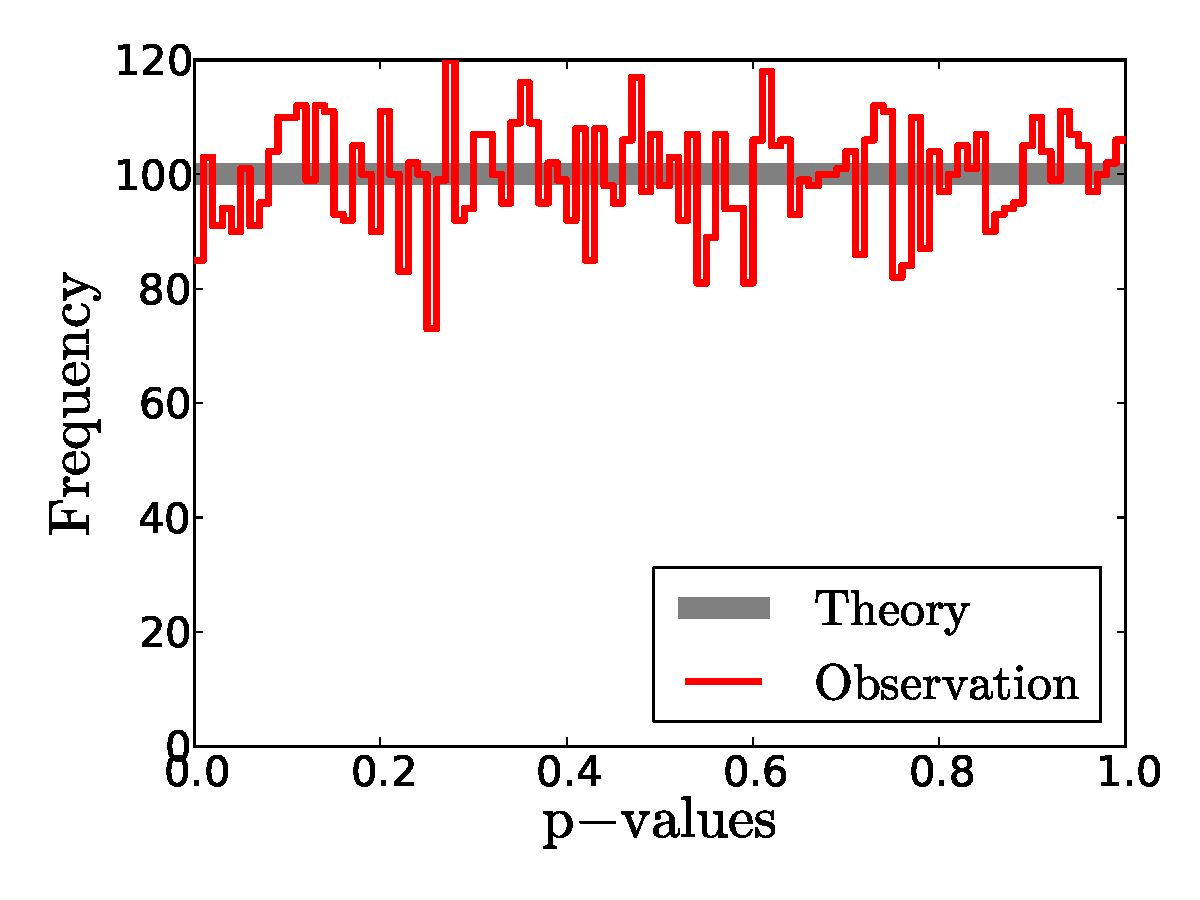
\includegraphics[width=\textwidth]{RCC_2_hist.pdf}
    \phantomcaption\label{subfig:RCC_hist_A}
\end{subfigure}
\begin{subfigure}[b]{0.49\textwidth}
	  \begin{flushleft}
	  \large B
		\end{flushleft}
    \centering
    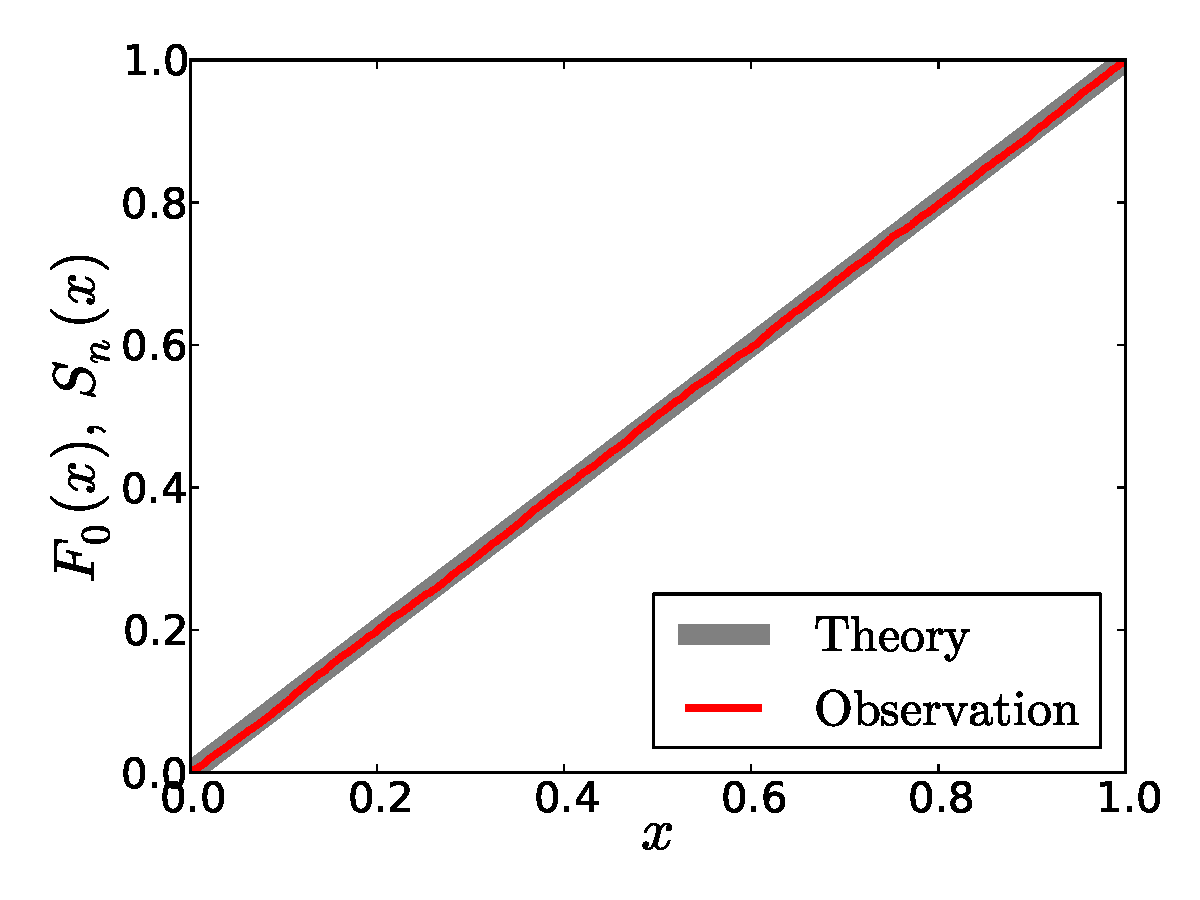
\includegraphics[width=\textwidth]{RCC_2_CDF.pdf}
    \phantomcaption\label{subfig:RCC_EDF_B}
\end{subfigure}
    \caption[Histogram and EDF of $p$-values from 10,000 chi-squared GOF tests]{\subref{subfig:RCC_hist_A}: Histogram of $p$-values from chi-squared goodness-of-fit tests of $n =$ 10,000 individual networks, combined into $100$ bins (red) together with the expected uniform distribution (grey). \subref{subfig:RCC_EDF_B}: The corresponding empirical distribution $S_n(x)$ (red) and expected cumulative distribution $F_0(x)$ (grey).}
  \label{fig:RCC_results_1}
\end{figure}

To assess the two-level testing procedure itself, it might be useful to be able to run it on data that we can safely assume to fulfill $H_0$. The test script allows us to do this with the optional argument \inline{control=True} passed to \inline{two_level_test}. NEST's connection algorithm is then swapped with a simple ``control algorithm'' that creates data that matches the multinomially distributed vector of degrees we would expect to get from NEST. It runs faster than the actual connection algorithm, and can therefore generate a larger data set in the same period of time. As mentioned briefly in Section \ref{sec:rcc}, the $p$-value from a chi-squared test is not truly a continuous variable. This distinctness might cause the two-level test to give a left-skewed distribution of $p$-values for certain combinations of parameters. The control algorithm can be used to investigate this. Running the two-level test procedure on the control algorithm, with $n_\text{runs}$ = 1,000, repeated $100$ times, each time with a different starting seed, yields the EDF of $p$-values in Figure \ref{fig:RCC_control_EDF}. These $p$-values appear to be uniformly distributed (a KS test of uniformity results in the $p$-value $0.468$). This is an important result, as the uniformity of the $p$-values from the two-level test procedure under $H_0$ is a prerequisite for drawing conclusions based on them.
\begin{figure}[h]
  \centering
  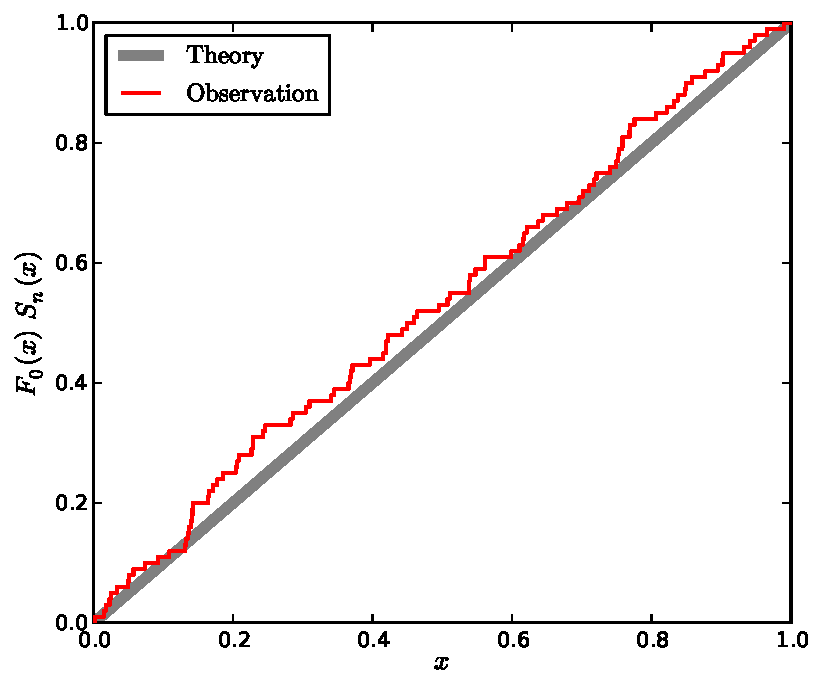
\includegraphics[width=0.8\textwidth]{RCC_control_EDF.pdf}
  \caption[EDF of 100 $p$-values from the two-level tests procedure]{EDF of 100 $p$-values from two-level test procedure. For each run, the two-level test procedure generates $n =$ 1,000 networks using the control algorithm, runs a chi-squared GOF tests on the vector of degrees, and tests the resulting $p$-values for uniformity using the KS test.}
  \label{fig:RCC_control_EDF}
\end{figure} 

The jumps of the chi-squared $p$-value will be large when the expected out-degree $N_\text{t} C / N_\text{s}$ is small, i.e., for small $N_\text{t}$ and $C$, and large $N_\text{s}$. The effect of small degrees is investigated. 
\begin{figure}[h]
  \centering
\begin{subfigure}[b]{0.49\textwidth}
	  \begin{flushleft}
	  \large A
		\end{flushleft}
    \centering
    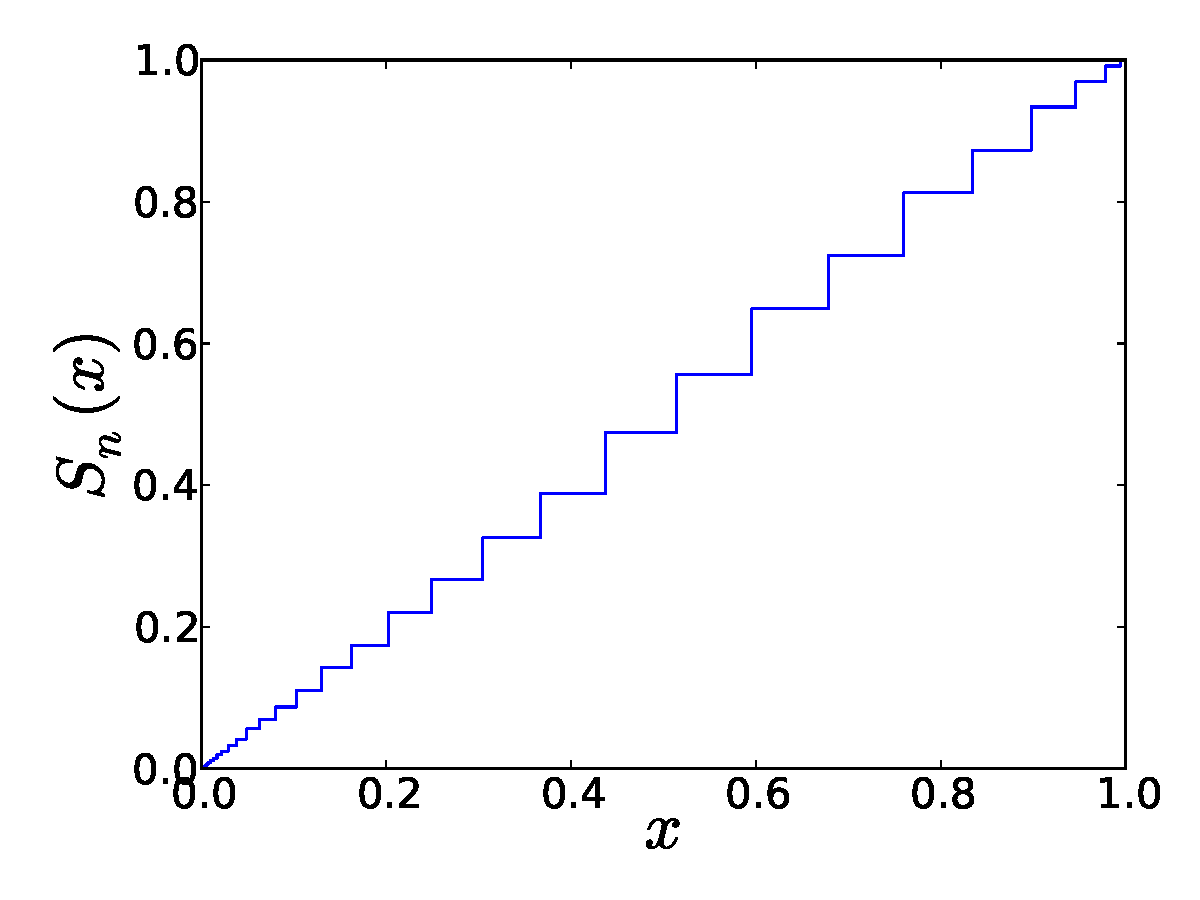
\includegraphics[width=\textwidth]{RCC_distinct_A.pdf}
    \phantomcaption\label{subfig:RCC_distinct_A}
\end{subfigure}
\begin{subfigure}[b]{0.49\textwidth}
	  \begin{flushleft}
	  \large B
		\end{flushleft}
    \centering
    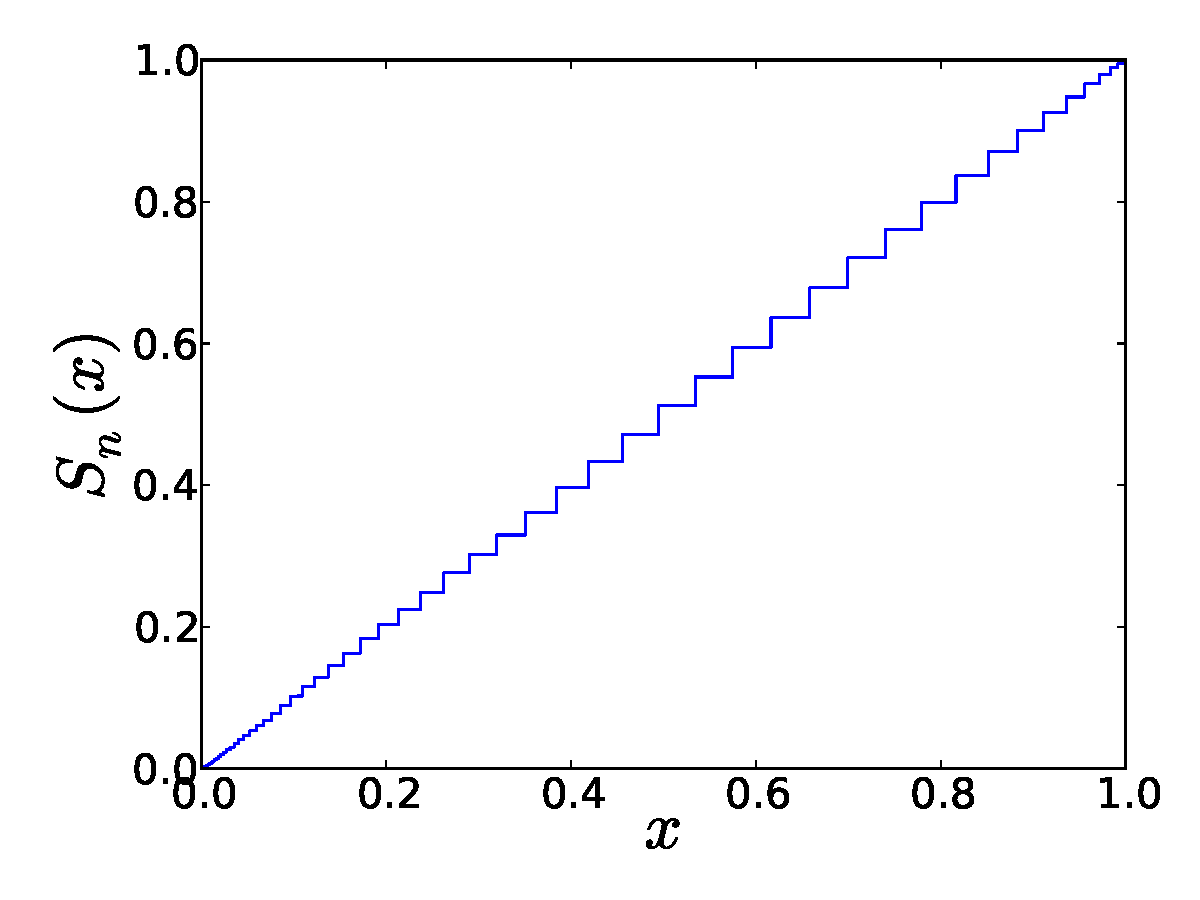
\includegraphics[width=\textwidth]{RCC_distinct_B.pdf}
    \phantomcaption\label{subfig:RCC_distinct_B}
\end{subfigure}
\\
\begin{subfigure}[b]{0.49\textwidth}
	  \begin{flushleft}
	  \large C
		\end{flushleft}
    \centering
    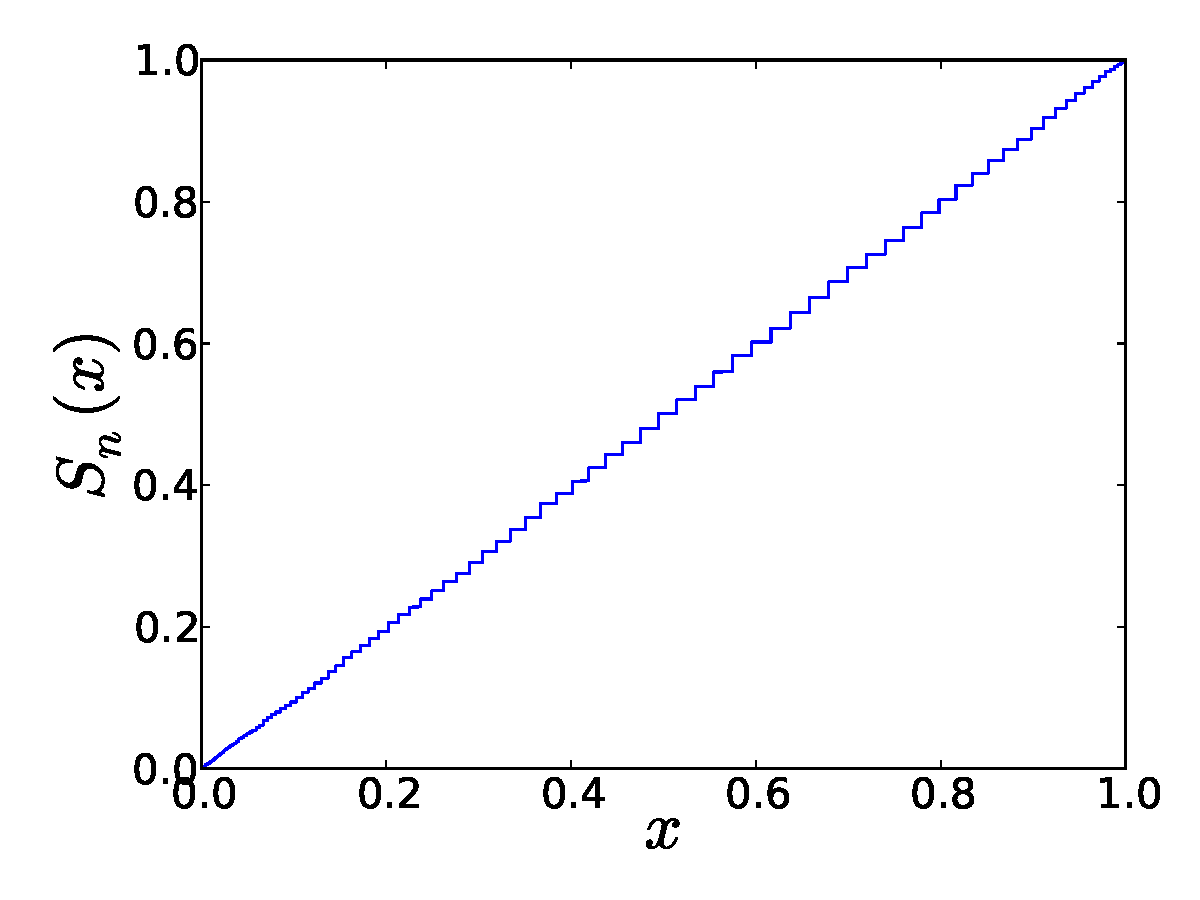
\includegraphics[width=\textwidth]{RCC_distinct_C.pdf}
    \phantomcaption\label{subfig:RCC_distinct_C}
\end{subfigure}
\begin{subfigure}[b]{0.49\textwidth}
	  \begin{flushleft}
	  \large D
		\end{flushleft}
    \centering
    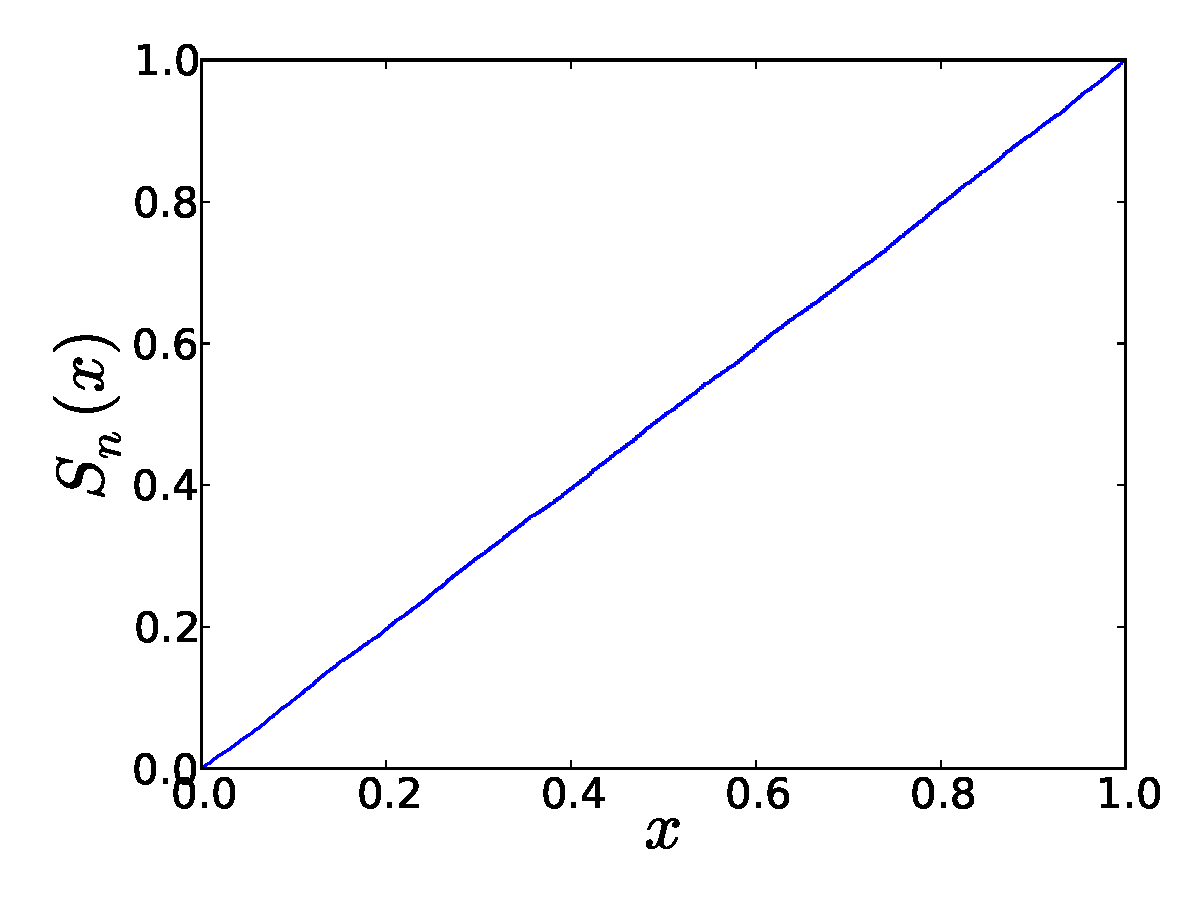
\includegraphics[width=\textwidth]{RCC_distinct_D.pdf}
    \phantomcaption\label{subfig:RCC_distinct_D}
\end{subfigure}
    \caption[The effect of small parameter values on the EDF of $p$-values]{EDFs of 10,000 $p$-values from chi-squared tests with four different combinations of values for the parameters $N_\text{s}$, $N_\text{t}$, and $C$. In \subref{subfig:RCC_distinct_A}, $N_\text{s} = 10$, $N_\text{t} = 5$, and $C = 5$, resulting in an expected out-degree of $2.5$. The $p$-values are clearly distinct, with fairly large jumps between adjacent values, especially for medium to large values. In \subref{subfig:RCC_distinct_B}, $N_\text{s} = 10$, $N_\text{t} = 10$, and $C = 5$. This gives an expected degree of $5$, resulting in smaller jumps. In \subref{subfig:RCC_distinct_C}, $N_\text{s} = N_\text{t} = C = 10$, resulting in an expected degree of $10$, and the jumps are smaller yet. In \subref{subfig:RCC_distinct_D}, $N_\text{s} = 10$, $N_\text{t} = 100$, and $C = 10$, giving an expected degree of $100$. The jumps are no longer visible.}
  \label{fig:RCC_distinct}
\end{figure}
Figure \ref{fig:RCC_distinct} shows the EDF of $p$-values with four different combinations of small values for these parameters. Jumps in the $p$-values are clearly seen. As expected, the jumps grow larger with a smaller expected out-degree. The $p$-values from the two-level test corresponding to the EDFs in Figure \ref{subfig:RCC_distinct_A}, \ref{subfig:RCC_distinct_B}, and \ref{subfig:RCC_distinct_C}, are $2.47\times 10^{-25}$, $6.47\times 10^{-5}$, and $0.0162$, respectively. These $p$-values are clearly left-skewed, even though the data tested does fulfill $H_0$. In the last figure, \ref{subfig:RCC_distinct_D}, the expected degree is $100$, and the $p$-value resulting from the two-level test is $0.237$. Re-running multiple times reveals that the fraction of $p$-values below $\alpha$ is close to $\alpha$. Thus, an expected degree of about $100$ seems to suffice to produce $p$-values that can be used to draw meaningful conclusions. 

Note that even though the two-level test will result in left-skewed $p$-values for small expected degrees, the fraction of $p$-values from a chi-squared test that lie below some level of significance $\alpha$ will be very close to $\alpha$, partly because the biggest jumps of the EDF are in the middle region, while in the lower part, close to $0$, the curves are fairly smooth (see Figure \ref{fig:RCC_distinct}). In other words, a two-level test might not be reliable for small expected degrees ($\lesssim 100$), but a ``one-level'' chi-squared test can be used with much smaller expected degrees ($\sim 5$).



\subsubsection{Sensitivity}

To assess the sensitivity of the two-level test procedure, i.e., its ability to detect small errors and biases, various errors and biases were deliberately introduced into the data. Some of these are described below, as well as the resulting $p$-values. We emphasize that these $p$-values are only examples. Rerunning the tests with the same biased algorithm and the same parameters, but with a different PRNG seed value, will result in a different $p$-value, possibly one that differs by quite a bit. Thus, they are only meant to give an indication of how well the bias is detected. 
Unless otherwise stated, the parameter values listed in Table \ref{tab:default_params_rcc_sensitivity} are used.

\begin{table}[h]
\begin{tabularx}{\linewidth}{| l | X | X | X | X | l | l |}
\hline
\cellcolor{Black}\textcolor{White}{\bf{Parameter}} & $N_\text{s}$ & $N_\text{t}$ & $C$ & $n_\text{runs}$ & \inline{start_seed} & \inline{control} \\ \hline
\cellcolor{Black}\textcolor{White}{\bf{Value}} & 1,000 & 1,000 & 100 & 1,000 & 0 & \inline{True} \\ \hline
\end{tabularx}
\caption[Default parameter set for sensitivity testing]{Default parameter set for sensitivity testing.}\label{tab:default_params_rcc_sensitivity}
\end{table}

The first bias that was deliberately introduced was a simple right-skewing of the data. The degree of the first half of the nodes was reduced by one, and the degrees of the second half was increased by one. This was easily detected by the test procedure ($p = 1.71 \times 10^{-5}$). In Figure \ref{fig:bias_example}, the distribution of 1,000 $p$-values are shown. It is clear from the figure that a single chi-squared test would not in any consistent way detect the bias. Only when we accumulate a large number of $p$-values is the trend obvious. 
\begin{figure}[b]
\centering
\begin{subfigure}[b]{0.49\textwidth}
	  \begin{flushleft}
	  \large A
		\end{flushleft}
    \centering
    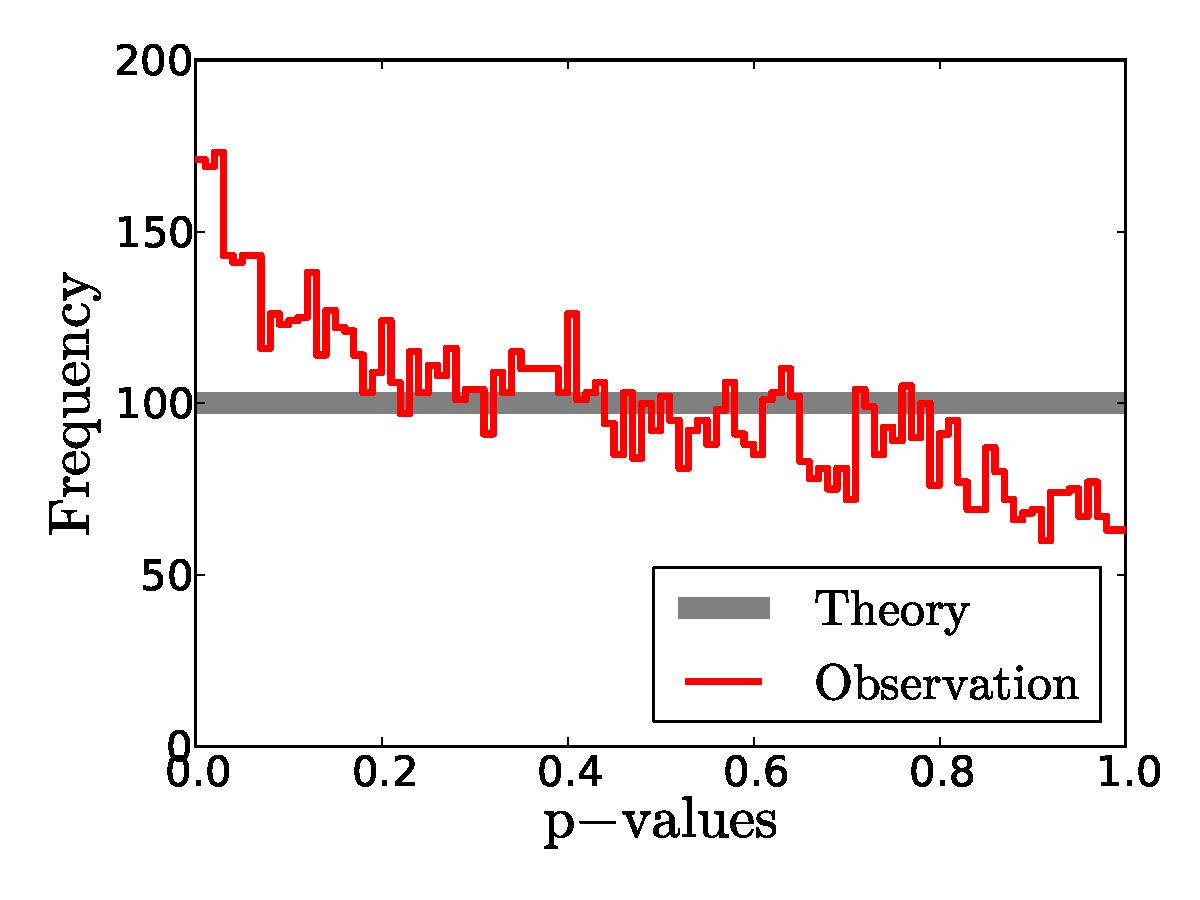
\includegraphics[width=\textwidth]{RCC_bias_hist.pdf}
    \phantomcaption\label{subfig:bias_hist}
\end{subfigure}
\begin{subfigure}[b]{0.49\textwidth}
	  \begin{flushleft}
	  \large B
		\end{flushleft}
    \centering
    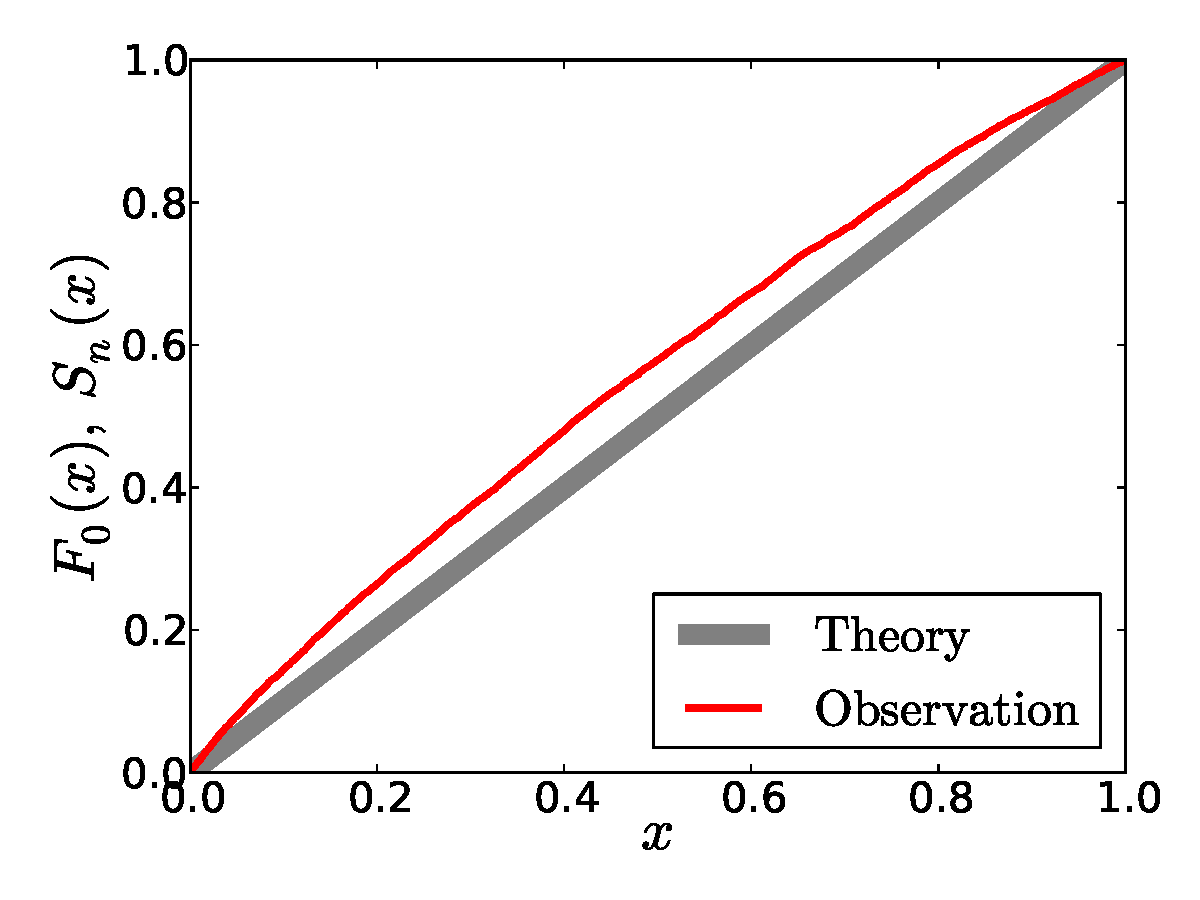
\includegraphics[width=\textwidth]{RCC_bias_CDF.pdf}
    \phantomcaption\label{subfig:bias_CDF}
\end{subfigure}
\caption[Distribution of $p$-values after introducing a bias into the connection algorithm]{Histogram (\subref{subfig:bias_hist}) and CDF (\subref{subfig:bias_CDF}) showing the distribution of $p$-values from chi-squared tests after introducing an error into the connection algorithm. Expectation is shown in grey.}
\label{fig:bias_example}
\end{figure} 

When $C$ was increased to 1,000, the bias was not detected ($p = 0.255$). A large $C$ is clearly not always advantageous for detecting small biases, especially biases that do not increase with $C$. Only after $n_\text{runs}$ was increased to 10,000 was the bias again detected ($p = 0.00428$). 

A second bias was introduced by decreasing the degree of every source node with an even-numbered index by one, and increasing the degree of every source node with an odd-numbered index by one. This was also easily detected ($p = 7.13 \times 10^{-6}$).

% Called bias 5, not 3, in biases.txt and test_RCC_bias.py.
A third bias was caused by increasing by one the degrees below the 5th percentile, and decreasing by one the degrees above the 95th percentile, thereby making the vector of frequencies a slightly ``too good'' fit to the theoretical distribution. This change was detected, both with $C = 100$ ($p = 8.02 \times 10^{-14}$) and $C =$ 1,000 ($p = 0.00231$), for $n_\text{runs} = 100$, as well as for larger $n_\text{runs}$. 

% Called bias 7, not 4, in biases.txt and test_RCC_bias.py.
A fourth bias was introduced by moving all the connections from one of the $N_\text{s}$ nodes to another node. This kind of error could easily be introduced by confusion between the zero-based numbering typically used in computer science and the one-based numbering used in everyday circumstances. The error was easily detected (the $p$-value was reported as $0.0$ as it was too small for Python's built-in floating point data type to handle). Increasing $N_\text{s}$ to 1,000, the error was still detected at $\alpha = 0.05$ ($p = 0.0366$).
	
% Called bias 3, not 5, in biases.txt and test_RCC_bias.py.
A fifth, very small bias was introduced by increasing the degree of one of the source nodes by one, and decreasing the degree of another node by one. The bias was not detected at $\alpha = 0.05$ with $C = 100$ and $n_\text{runs} =$ 10,000 ($p = 0.0740$), nor with $C$ reduced to 10. Reducing $N_\text{s}$ and $N_\text{t}$ to 100, the bias was detected at $\alpha = 0.05$ ($p = 0.0189$). A smaller network clearly increases the sensitivity to certain types of biases, especially biases that do not increase with network size.

Several similar tests were run. Generally the two-level test procedure seems quite sensitive to small biases. The sensitivity obviously increases with $n_\text{runs}$, but not necessarily with $C$, $N_\text{t}$ and $N_\text{s}$. The effect of these parameters on the sensitivity depends on the nature of the bias we wish to detect. It might therefore be a good idea to run the procedure with different  sets of parameters. 

\graphicspath{{figs/nonspatial/}}



\section{Random divergent connections\label{sec:rdc}}

\inline{RandomDivergentConnect} works in very much the same way as \linebreak \inline{RandomConvergentConnect}, except that the source nodes are now iterated over, and target nodes are randomly drawn and connected, meaning that the out-degrees of the source nodes are now all $C$, while the in-degrees of the target nodes will vary. It might therefore seem superfluous to test both functions. Running NEST with multiple VPs, however, the exact implementation of the connection algorithm is not the same for the two functions. This is because different nodes are handled by different VPs, and information about connections is handled by the same VP by which the \emph{target} node is handled \cite{plesser2007efficient}. To minimize the amount of inter-VP communication necessary, each VP is given its own PRNG. \inline{RandomDivergentConnect} uses the global PRNG when drawing connections, while \inline{RandomConvergentConnect} uses the per-VP PRNGs. The result is different connectivity patterns, even with the same master seed value. Both function should therefore be tested with multiple VPs.



\subsection{Implementation\label{subsec:rdcimp}}

The Python module for testing \inline{RandomDivergentConnect}, found in Appendix \ref{app:rdc}, is very similar to the module for testing \inline{RandomConvergentConnect}. A class \inline{RDC_tester}, with the two methods \inline{chi_squared_test} and \inline{two_level_test}, is defined. These methods take the same parameters as their counterparts in the convergent case. As before, the usage is demonstrated in the main section of the module.



\subsection{Results\label{subsec:res_rdc}}

\graphicspath{{figs/nonspatial/RDC_results/}}

Running the script in in Appendix \ref{app:rdc} with the same parameter set used for random convergent connections, listed in Table \ref{tab:default_params_rcc_results}, results in a $p$-value of $0.905$. This matches exactly the $p$-value we got in Section \ref{subsec:res_rcc} after running the test script in Appendix \ref{app:rcc} with the same set of parameters. In fact, the distribution of connections among source nodes for a network created by \inline{RandomConvergentConnect} will exactly match the distribution \linebreak of connections among target nodes for a network created by \linebreak\inline{RandomDivergentConnect}, when NEST is run with one VP. For multiple VPs, however, the resulting distribution of connections is not the same. The test class in the test script can be instantiated with the additional argument \inline{threads}, causing NEST to operate with the specified number of local threads. With NEST running as a single process, the number of VPs will equal the number of local threads. Running the script in Appendix \ref{app:rdc} with the same parameter set as before (listed in Table \ref{tab:default_params_rcc_results}), but with the extra argument \inline{threads = 2}, the we obtained a $p$-value of 0.931, consistent with the expected multinomial distribution of in-degrees.

\graphicspath{{figs/nonspatial/}}



\section{Automated test procedure\label{sec:auto}}

We will now describe how to turn a variant of the test procedure described in the previous sections into an automated test, implemented as a unit test. This places some practical limitations on the test procedure. The test must not take too long to run. It should also not have a too high rate of false positives (type I error). At the same time we do of course not want to loose too much sensitivity. 

A quick and efficient approach would be to generate one single network and run a chi-squared test on the distribution of connections with some relatively low level of significance $\alpha$, say, $0.01$, as described earlier, but even with this low level of significance, we would still see false positives for about 1\% of the test runs. Reducing $\alpha$ further would result in a lower sensitivity. On the other hand, running the more thorough but slow two-level test procedure described in Section \ref{sec:rcc} every time is quite time-consuming. Instead, an adaptive approach is proposed here, similar to the one used by \citeN{lecuyer2007testu01}. First, a single network is generated, and a chi-squared test is performed on the distribution of connections. If the resulting $p$-value is deemed too extreme, a larger number $n_\text{runs}$ of networks is generated, and a more thorough two-level test is performed, either confirming or allaying our suspicion. This will allow us to require a fairly high level of significance for the chi-squared test, thereby keeping the sensitivity high, while at the same time having a low rate of false positives.

As was shown in Section \ref{subsec:res_rcc}, not all errors and biases are best detected with a large network or with large degrees, as this might hide certain types of small biases. Tests should therefore be run with different values of $N_\text{s}$, $N_\text{t}$, and $C$. For a single chi-square test, the network can be quite small, and the only limit is that the expected degree must not be below $e_\text{min}$, but the two-level test procedure is more sensitive, and the expected degree should not be much lower than 100. Both \inline{RandomConvergentConnect} and \inline{RandomDivergentConnect} should be tested. Running tests both with a single VP and with multiple VPs might also be a good idea, as the implementation of the connection algorithms are somewhat different for multiple VPs (see Section \ref{sec:rdc}).

For the $p$-values from the chi-squared test, both very low and very high values are considered suspicious. Let $\alpha_{1,\text{lower}}$ and $\alpha_{1,\text{upper}}$ be the values below and above which, respectively, $p$-values are deemed suspicious. Under $H_0$, suspicious values will occur for a fraction $\alpha_1 = \alpha_{1,\text{lower}} + \left(1 - \alpha_{1,\text{upper}}\right)$ of the tests performed. Whenever such an extreme value is encountered, the two-level test is performed. Let $\alpha_2$ be the value below which the $p$-value from the KS test is considered too extreme, and $H_0$ is rejected. The total fraction of false positives will then be
\begin{equation}
\alpha = \alpha_1 \times \alpha_2 = \left( \alpha_{1,\text{lower}} + 1 - \alpha_{1,\text{upper}} \right) \times \alpha_2
\end{equation}
With $\alpha_{1,\text{lower}} = 0.025$, $\alpha_{1,\text{upper}} = 0.975$, and $\alpha_2 = 0.05$, $\alpha$ becomes $0.0025$. The choice of these critical values, as well as the test parameters ($N_\text{s}$, $N_\text{t}$, $C$, $n_\text{runs}$) will depend on the intended usage of the unit test, the computing power of the system it will run on, the maximum time the test can be allowed to take, the desired fraction of false positives, etc. 



\subsection{Implementation\label{subsec:autoimp}}

An implementation of the automated test procedure can be found in Appendix \ref{app:unit}. It is implemented using the Python unit testing framework \inline{unittest}. The test scripts for \inline{RandomConvergentConnect} and \inline{RandomDivergentConnect}, found in Appendix \ref{app:rcc} and \ref{app:rdc}, are imported to avoid code duplication. 

The test is repeated three times for each of \inline{RandomConvergentConnect} and \inline{RandomDivergentConnect}, once with a small network, once with a larger network, and once with multiple VPs, giving a total of six test cases. $n_\text{runs}$ can have different values for each test, as we might want to run a test on a small network a larger number of times than a test on a large network. The critical values are $\alpha_{1,\text{lower}} = 0.025$, $\alpha_{1,\text{lower}} = 0.975$, and $\alpha_2 = 0.05$. We thus expect a fraction $0.0025$ of the tests to fail. When running the test suite with the six test cases 500 times, giving a total of 3,000 test runs, 10 failures were encountered. This is close to the $\sim 0.0025\times3000 = 7.5$ false positives we would expect.

When the six one-level chi-squared tests are passed, the suite takes less than a minute to complete on most systems. In the event that all six one-level tests fail (which will happen with a probability of $0.05^{6} = 1.5625\times 10^{-8}$ under $H_0$), and the two-level test is invoked, the entire suite might take a few minutes to complete, depending on hardware, installed version of NEST etc. 



\clearchapter

